\documentclass[conference]{IEEEtran}
\usepackage{amsmath}
\usepackage{blindtext}
\usepackage{graphicx}
\usepackage[caption=false]{subfig}
\usepackage{import}
\usepackage{amsmath}
\usepackage{listings}
\usepackage{pdfpages}
\DeclareMathOperator*{\argmax}{arg\,max}
\DeclareMathOperator*{\argmin}{arg\,min}

\usepackage[hidelinks]{hyperref}
\hypersetup{
    breaklinks=true,
    bookmarksopen=true,
}


\def\BibTeX{{\rm B\kern-.05em{\sc i\kern-.025em b}\kern-.08em
    T\kern-.1667em\lower.7ex\hbox{E}\kern-.125emX}}


\renewcommand{\thefootnote}{\fnsymbol{footnote}}


\begin{document}

\title{Handwritten Digit Recognition Using Deep Convolutional Neural Network*}




\author{\IEEEauthorblockN{Ammar Elsabe}
\IEEEauthorblockA{
    U19100452@sharjah.ac.ae\\
    University ID: U19100452
}

\and

\IEEEauthorblockN{Mohamed Alzaabi}
\IEEEauthorblockA{
    U17105281@sharjah.ac.ae\\
    University ID: U17105281
}

\and

\IEEEauthorblockN{Abdulaziz Abdullatif}
\IEEEauthorblockA{
    U18103708@sharjah.ac.ae\\
    University ID: U18103708
}}

\maketitle
\begin{abstract}
    A Convolutional Neural Network (CNN) is a powerful tool for image classification.\@ However, despite existing since the late 1980s, they have been majorly dormant until the mid-2000s, which is when computing power and large databases of labeled data started becoming more accessible thanks to GPU technology and the internet, respectively.\@ This paper pits the use of a Deep Convolutional Neural Network (DCNN) against the MNIST database of handwritten digit images, and as will be seen by the end of the paper, the performance of these networks on a (cheap, consumer) GPU is simply a marvel of engineering, nearing human--level accuracy.
\end{abstract}

\section{Introduction}
\footnotetext[1]{Code can be found at \href{https://github.com/ammar-elsabe/handwritten-digit-recognition-DCNN.git}{\texttt{github.com/ammar-elsabe/handwritten-\\digit-recognition-DCNN.git}}}
Deep learning can now be applied to a growing variety of industries. Convolutional Neural Networking (CNN) is a deep learning technique for evaluating visual data. Convolutional Neural Networking can be used for object detection, face recognition, robotics, sound detection and recognition, video analysis, clustering, pattern recognition, language processing, weather prediction, spam detection, topic categorization, regression analysis, speech recognition, image classification, and handwritten digit recognition.
 Object Character Recognition (OCR) is one of the influencing projects that has used deep learning (Object Character Recognition). OCR is a method of converting printed or written characters into encoded text. The OCR tool scans a document and extracts the information, which is then saved as a digital document. OCR may be implemented in two ways: one by identifying patterns in the characters, and the other by segmenting the text. In any case, machine learning is oblivious to this issue. Handwritten digit recognition (HDR) is a subset of OCR that recognizes digits rather than the entire character's data. HDR is a lighter and quicker alternative to OCR.\@ HDR has a lot of flexibility in areas like medicine, finance, student administration, and the taxes procedure.
Handwritten digit recognition (HDR) refers to a computer's ability to recognize human handwritten digits from a variety of sources, such as photographs, papers, and touch displays, and classify them into ten specified categories (0--9). In the area of deep learning, this has been a topic of inexhaustible investigation. Numerous applications exist for digit recognition, including number plate identification, postal mail sorting, and bank check processing. Because handwritten digit identification is not an optical character recognition, we encounter several obstacles due to the various styles of writing used by different people. A human brain can simply analyse and extract data from a complex image, but for a computer, an image is just a collection of pixels, which are nothing more than a list of values ranging from 0 to 255, with blends such as RGB, B.W., greyscale, etc. Pixel values can be used to extract information from a picture.
This paper experiments with a simple Deep Convolutional Neural Network on the MNIST\cite{6296535} dataset to evaluate their performance.\@ We delve into Convolutional Neural Networks in detail in Section \ref{sec:cnn} as a preliminary to describing the simple architecture used in Section \ref{sec:train}, and we evaluate the the model's performance in Section \ref{sec:test}.

\section{The MNIST Dataset}
The Modified National Institute of Standards and Technology (MNIST) database is a database of handwritten digits \cite{6296535} that is a classic benchmark for image recognition.\@ It is also widely used in the machine learning world\cite{Platt1998}.\@ It consists of a training set of 60,000 images and a test set of 10,000 images.\@ The training set is used to train the network, and the test set is used to evaluate its performance.\@ The images are $28 \times 28$ pixels, and the labels are 0 to 9. It is a subset of a larger set available from NIST.\@ It was created in 1998 as a combination of two of their databases, Special Database 1 and 3, which contained digits written by high school students and empoyees of the United States Census Bureau, respectively.\@ Half of the database was taken from ``Special Database 1'', and the other half was taken from ``Special Database 3''. The original creators kept a list of the methods tested on it\cite{726791, mnist}, and in their original paper they used a Support Vector Machine (SVM) to achieve an accuracy of 99.2\%\cite{1265868}.
\par
There exists another database called Extended MNIST (EMNIST) created to the successor to MNIST\cite{emnist} created from NIST ``Special Database 19'', which includes the handwritten uppercase and lowercase letters, as well as digits.\cite{emnist2} EMNIST was created only using the digits subset of ``Special Database 19''. In the following sections of this paper, we use MNIST (not EMNIST) for our CNN.\@

\begin{figure}[!htp]
    \includegraphics[width=\columnwidth]{./figs/mnist.png}
    \caption{Examples from the MNIST dataset}\label{fig:mnist}
\end{figure}

\section{Convolutional Neural Networks}\label{sec:cnn}
Convolutional Neural Networks (CNNs) are compriesd of an input layer, hidden layers and an output layer. As with any feed-forward neural network, the middle layers are reffered to as hidden layers because their inputs and outputs are masked by the activation function and final convolution. In a CNN, these hidden layers include layers that perform convolutions, which usually involves computing a dot product of the convolution kernel and the layer's input matrix. The convolution operation generates a feature map as the convolution kernel slides along the input matrix for the layer, which then contributes to the input of the next layer. Other layers such as pooling layers, fully connected layers, and normalization layers are then added.
\subsection{Convolutional Layers}
The input to a CNN is a tensor with the following shape: (number of inputs) x (input height) x (input width) x (input channels). After passing through a convolutional layer, the image is abstracted to a feature map, also known as an activation map, with the following shape: (number of inputs) x (feature map height) x (feature map width) x (feature map channels).
\par Convolutional layers convolve the input and pass the result to the following layer. This is analogous to a neuron's response to a specific stimulus in the visual cortex.

\subsection{Pooling Layers}
Along with traditional convolutional layers, convolutional networks may include local and/or global pooling layers. By combining the outputs of neuron clusters at one layer into a single neuron in the next layer, pooling layers reduce the dimensions of data. Local pooling combines small clusters, with tiling sizes as small as $2 \times 2$ being common. Global pooling affects all neurons in the feature map\cite{inproceedings, article2}. There are two types of pooling that are commonly used: maximum and average. The maximum value of each local cluster of neurons in the feature map is used in max pooling\cite{yamaguchi1990neural, 6248110}, while the average value is used in average pooling.

\subsection{Fully Connected Layers}
Layers that are fully connected connect every neuron in one layer to every neuron in the next layer. It functions similarly to a traditional multilayer perceptron neural network (MLP). To classify the images, the flattened matrix is passed through a fully connected layer.
%\pagebreak
\section{Training the model}\label{sec:train}
We used Google's TensorFlow API\cite{tensorflow2015-whitepaper} in Python to train the model on a consumer computer with the following specefications:
\begin{itemize}
    \item CPU:\@ Intel i5--8400
    \item GPU:\@ NVIDIA GeForce GTX 1060
    \item RAM:\@ 16GB
\end{itemize}
\begin{figure}[!htp]
    \centering
    \def\svgwidth{\columnwidth}
    \scriptsize
    \import{./figs/}{cnn_architecture.pdf_tex}
    \caption{The CNN architecture used to train the model}\label{fig:cnn_architecture}
\end{figure}
Instead of preprocessing the data, we elected to not preprocess the data at all (except for some automatic tuning and batching to speed up the training), but to have the model take the raw grayscale $28 \times 28$ pixel images.\@ We decided to do that in order to show how powerful DCNNs can be and how good they can be at feature extraction.\@
As such, our neural network (Figure \ref{fig:cnn_architecture}) starts with a rescaling layer, which is nothing but normalizing the grayscale values from $[0, 255]$ to $[0, 1]$. It is then followed by a 2D convolutional layer with $28 \, 3 \times 3$ kernels, outputting 28 feature maps. The feature maps are then pooled with a $2 \times 2$ pool--size max pooling layer, cutting the amount of pixels in each feature map by $4$. We then apply batch normalization\cite{batchnorm} to reduce overfitting, and redo the above process once more before flattening the image.\@
Following the flattening of the feature maps, we are left with a 1 dimensional vector of size 700, which is then inputted to a series of fully connected layers, with the number of perceptrons in each layer going $700 \to 128 \to 128 \to 10$. All the layers in the neural network used the relu activation function, except the last one which uses softmax to output its predictions.
The loss function used was categorical crossentropy, which is:
\begin{equation}
    J(\textbf{w}) = -\frac{1}{N} \sum_{i=1}^{N} \left[ y_i \text{log}(\hat{y}_i) + (1-y_i) \text{log}(1-\hat{y}_i) \right]
\end{equation}
and the optimizer used was the ``Adam'' optimizer, which is a version of Stochastic Gradient Descent (SGD)\cite{adam} that we hyperparameterized with the default learning rate of $0.001$
%The architecture used is shown in Figure \ref{fig:cnn_architecture}.  
The callbacks used were the following:
\begin{lstlisting}[language=Python]
tf.keras.callbacks.EarlyStopping( 
    monitor="val_loss",
    patience=5,
),
tf.keras.callbacks.ModelCheckpoint( 
    "model.h5",
    monitor="val_loss",
    save_best_only=True,
    verbose=1
)
\end{lstlisting}
That is to say that training stops once it plateaus (with 5 epochs and no improvement), and that we save the best performing model (in terms of validation loss), which we later load and use for the predictions.\@ With our architecture and even our cheap, widely available specifications, training took merely a minute, and the per--epoch progress is shown in Figure \ref{fig:perepoch}
\begin{figure}[!htp]
    \centering
    \scriptsize
    \subfloat[Training and validation accuracy\label{performance:accuracy}]{
        \def\svgwidth{0.5\columnwidth}
        \import{./figs/}{accuracy.pdf_tex}
    }
    \subfloat[Training and validation loss\label{performance:loss}]{
        \def\svgwidth{0.5\columnwidth}
        \import{./figs/}{loss.pdf_tex}
    }
    \caption{The per--epoch progress of the model's performance }\label{fig:perepoch}
\end{figure}
\par From Figure \ref{fig:perepoch}, we can see that the model reaches a high, near--human accuracy, but following the first epoch the rate of improvement decreases, and following the third epoch it begins to overfit, where the training loss and accuracies are steadily improving but the validation training and loss are in fact getting \textit{worse}.

\section{Model Evaluation}\label{sec:test}
Following training the model, we can define the trained model mathematically as a bayesian probability distribution over the 10 classes: $\hat{p}(y | x)$; the probability of a label $y$ given an image $x$.
Testing the model on the test set nets us with a 2D matrix $a$, with $10000$ rows and $10$ columns.\@ The $i$\textsuperscript{th} row corresponds to the $i$\textsuperscript{th} image in the test set, and the $j$\textsuperscript{th} column corresponds to a digit $j$.\@ The value of $a_{i,j}$ is the probability that the $i$\textsuperscript{th} image contains the $j$\textsuperscript{th} digit, or mathematically:
\begin{equation}
    a_{i,j} = \hat{p}(y = j | x = i)
\end{equation}
We define the predicted label for an image $i$ as the label with the highest probability outputted by the model:
\begin{equation}
    y_i = \argmax_j a_{i,j}
\end{equation}
Where $y$ is the set of predicted outputs. Let $x$ be the set of actual labels, and let $C_{sd}$ be the set of images belonging to the digit $d$ in the set $s$ (for example: $C_{y0}$ is the set of images that are predicted to be 0/labeled as 0 in the set $y$):
\begin{equation}
    C_{sd} = \{i \in \{1, 2, \;\ldots, 10000\} : s_i = d\}
    \;\label{eq:setofimages}
\end{equation}
\par A confusion matrix, also known as an error matrix, is a square matrix of size $n \times n$ where $n$ is the number of classes. It is a specifici table layout that allows the visualization of a model's performance. Each row of the matrix represents the instances in an actual class, while each column represents the instances in a predicted class\cite{Stehman1997}. With $C$ defined in (\ref{eq:setofimages}), we can mathematically denote the confusion matrix as:
\begin{equation}
    %\scriptstyle
    M = \begin{bmatrix}
        |C_{x0} \cap C_{y0}| & |C_{x0} \cap C_{y1}| & \cdots & |C_{x0} \cap C_{y9}| \\
        |C_{x1} \cap C_{y0}| & |C_{x1} \cap C_{y1}| & \cdots & |C_{x1} \cap C_{y9}| \\
        \vdots & \vdots & \ddots & \vdots \\
        |C_{x9} \cap C_{y0}| & |C_{x9} \cap C_{y1}| & \cdots & |C_{x9} \cap C_{y9}|
    \end{bmatrix}
\end{equation}
Plotting $M$ on a heatmap, we can see the confusion matrix in Figure \ref{fig:confusion_matrix}.
\begin{figure}[!htp]
    \centering
    \def\svgwidth{\columnwidth}
    \scriptsize
    \import{./figs/}{confusion_matrix.pdf_tex}
    \caption{Confusion matrix of the trained model}\label{fig:confusion_matrix}
\end{figure}
\par With the confusion matrix computed, we can define accuracy as the following equation using the confusion matrix:
\begin{equation}
    \text{accuracy} = \frac{\sum_{i = 0}^9 k_{ii}}{\sum_{i = 0}^9 \sum_{j = 0}^9 k_{ij}} \times 100
\end{equation}
where $k_{xy}$ represents an element in the $x^\text{th}$ row and $y^\text{th}$ column of the confusion matrix, in other words it is the sum of the elements in the diagonal of the confusion matrix (correct predictions), dividied by the total sum (total number of samples in the dataset). Calculating the values nets us a diagonal sum of $9908$, and since the test split of the MNIST dataset is $10000$ images, that gives us an accuracy of $99.08\%$.
\par
We can also calculate the per--digit accuracy of a digit $i$ as:
\begin{equation}
    \text{accuracy}_{i} = \frac{k_{ii}}{\sum_{j = 0}^9 k_{ij}} \times 100
\end{equation}
which gives us the values needed to plot the accuracy of each digit in the bar chart shown in Figure \ref{fig:bar}.
\begin{figure}[!htp]
    \centering
    \def\svgwidth{\columnwidth}
    \import{./figs/}{bar_plot.pdf_tex}
    \caption{The accuracy of the model at detecting each digit}\label{fig:bar}
\end{figure}
\par From the bar chart, we can see that the highest accuracy is achieved by the model detecting the digit $4$ at an accuracy of $99.8982\%$, and the lowest accuracy is detecting the digit $9$ with an accuracy of $98.1169\%$.
\section{Conclusion}
In conclusion, we believe that DCNNs have an important role in upcoming OCR technologies.\@ The results of our experiment are phenomonal, near--human accurate, and with very little cost in terms of time spent on developing the model, training the model, and the price of the hardware used.\@

\bibliographystyle{IEEEtran}
\bibliography{paper.bib}

\onecolumn

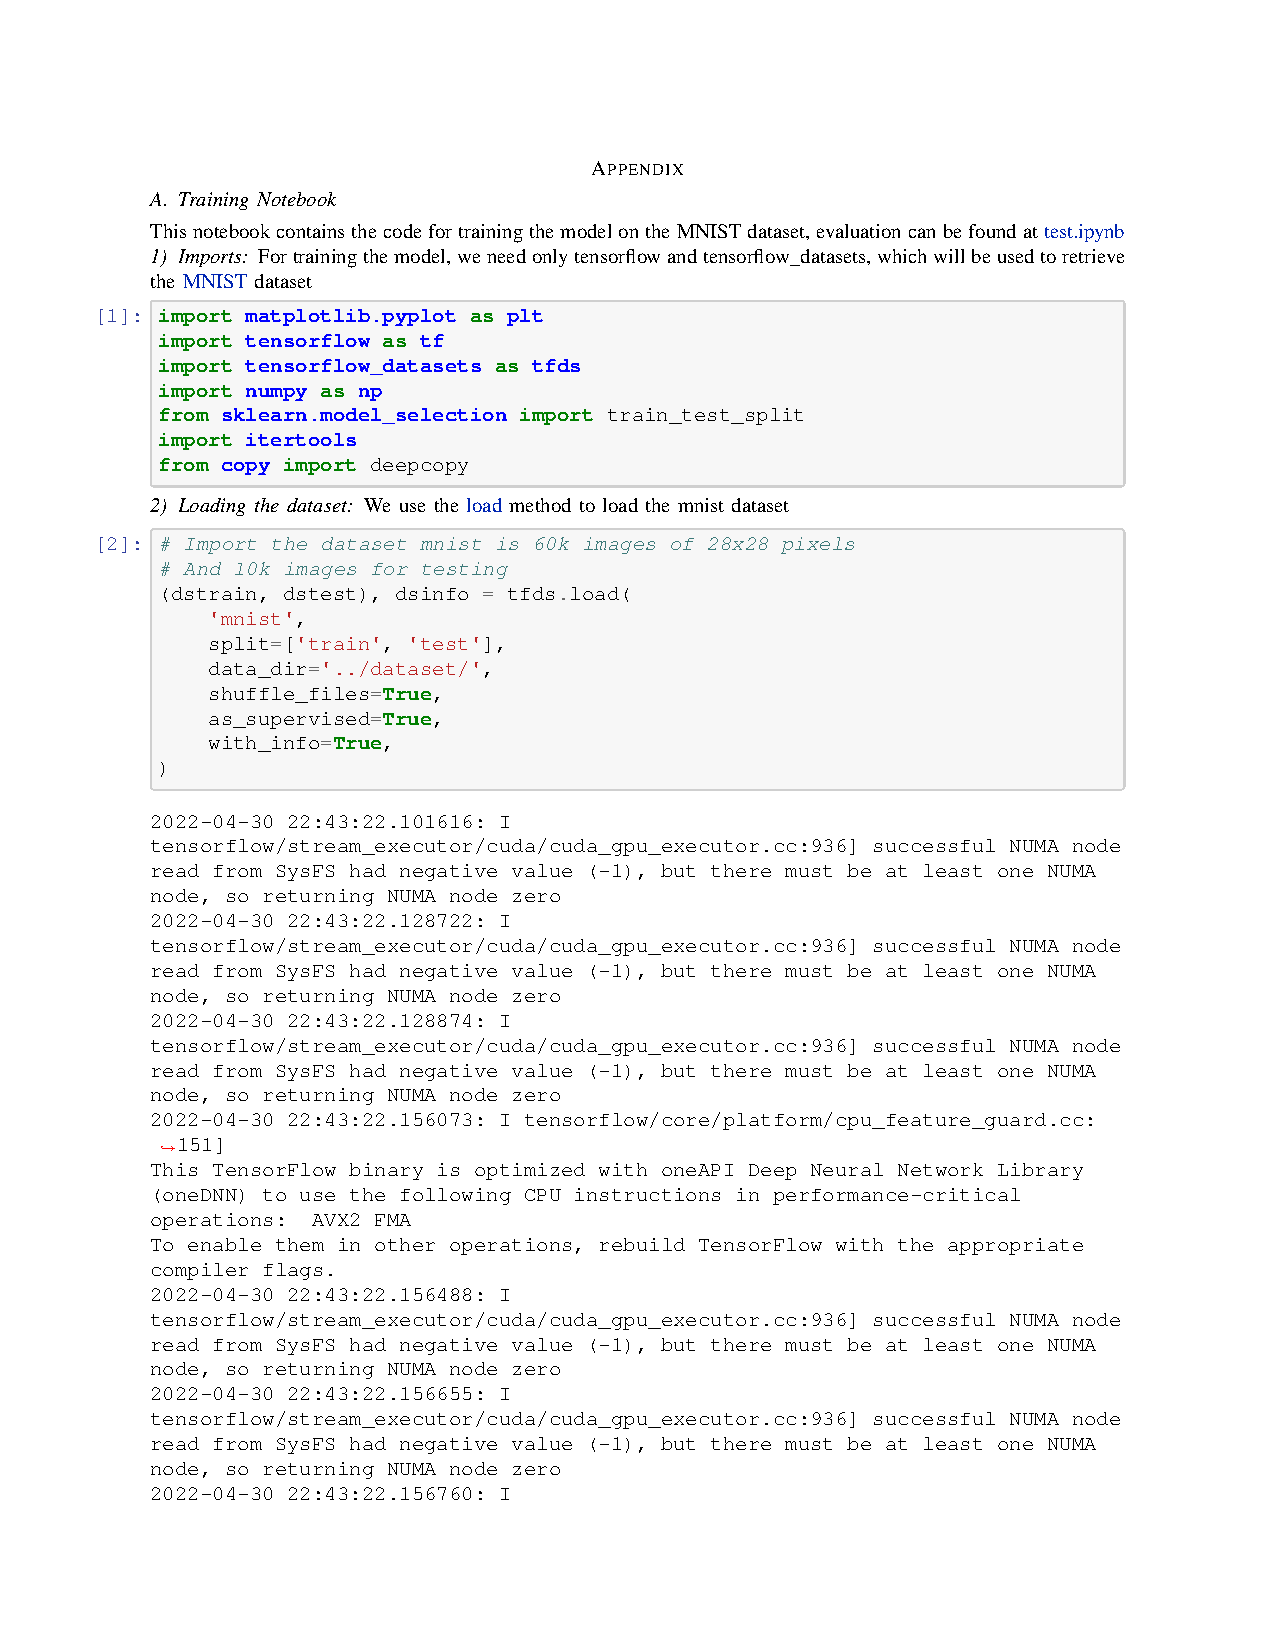
\includepdf[pages=-, addtotoc={
    1,section,1,Appendix,Appendix,
    1,subsection,2,Training Notebook,train}]
    {./appendix/train.pdf}
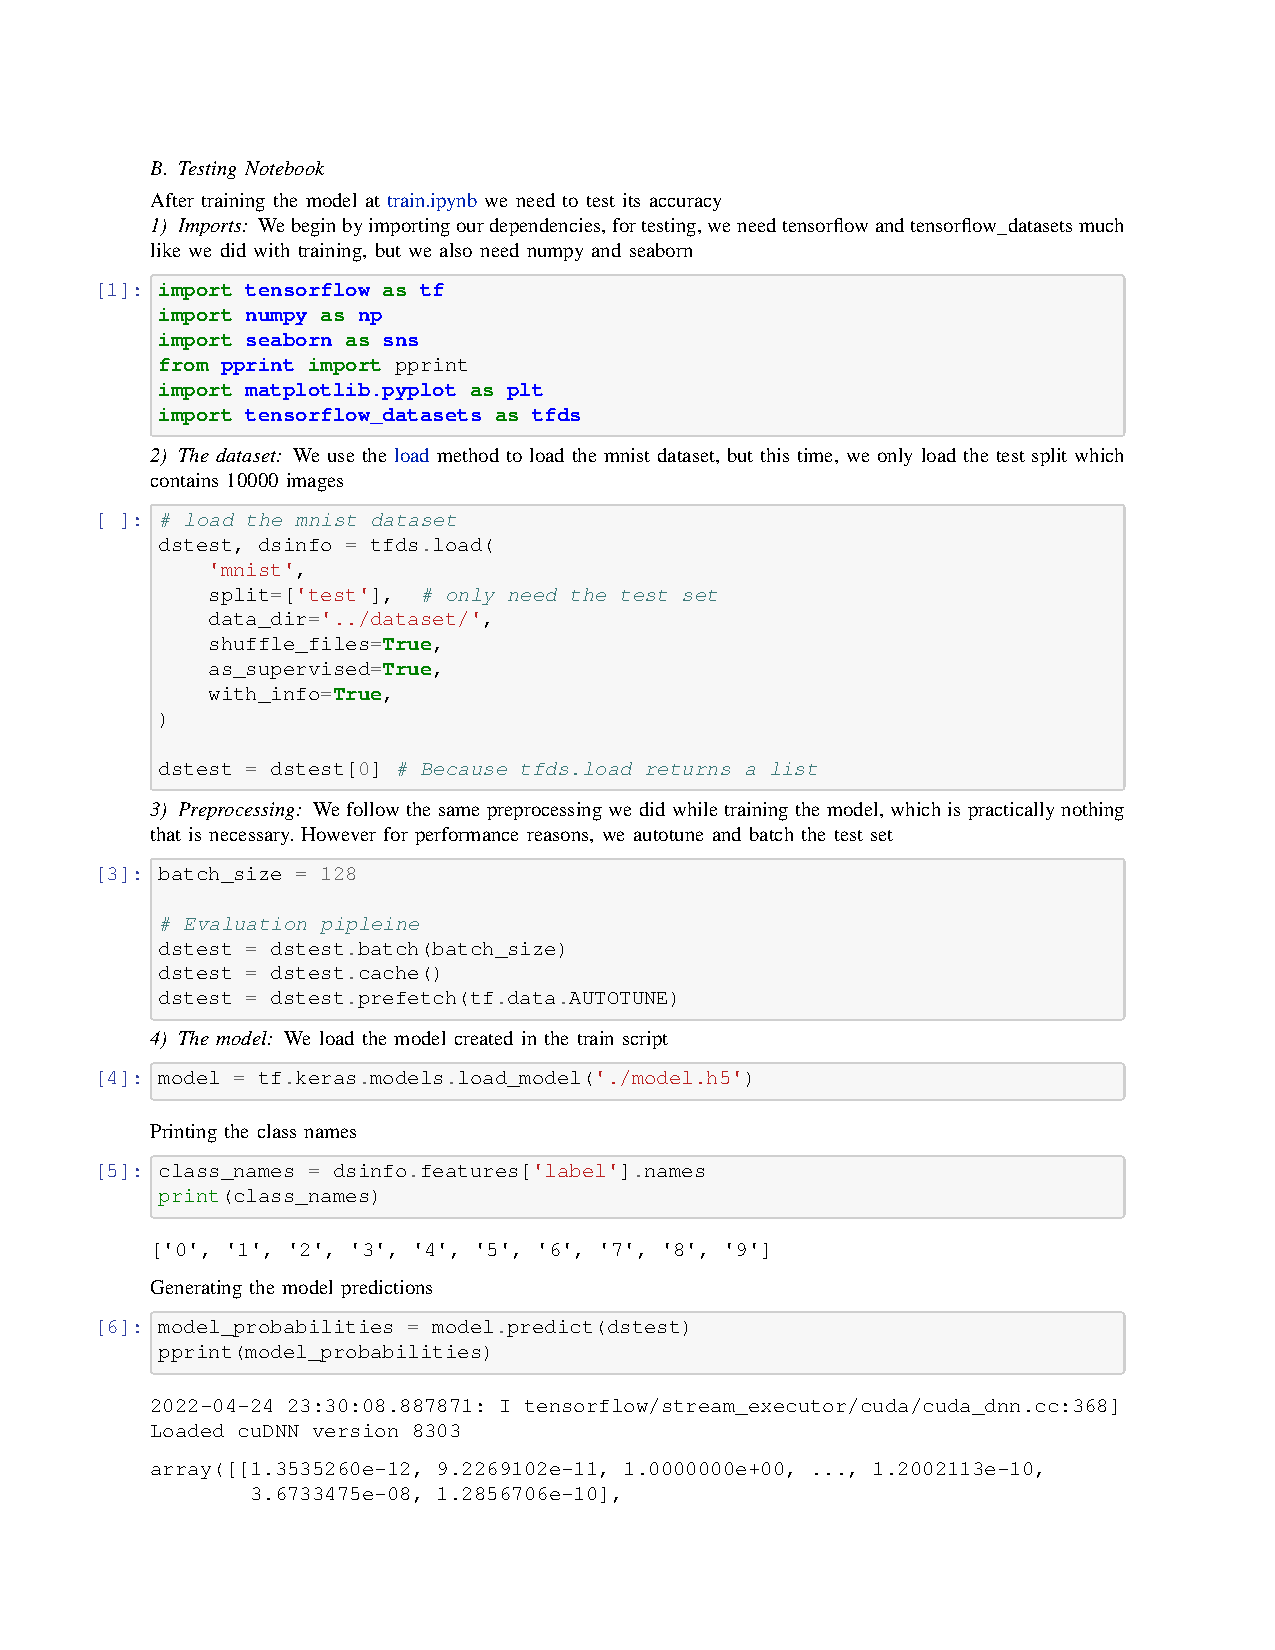
\includepdf[pages=-, addtotoc={
    1,subsection,2,Testing Notebook,test}]
    {./appendix/test.pdf}

\end{document}
